\documentclass[a4paper]{article}
\usepackage[utf8]{inputenc}
\usepackage[spanish, es-tabla, es-noshorthands]{babel}
\usepackage[table,xcdraw]{xcolor}
\usepackage[a4paper, footnotesep = 1cm, width=22cm, top=2.5cm, height=25cm, textwidth=20cm, textheight=25cm]{geometry}
%\geometry{showframe}

\usepackage{tikz}
\usepackage{amsmath}
\usepackage{amsfonts}
\usepackage{amssymb}
\usepackage{float}
\usepackage{graphicx}
\usepackage{caption}
\usepackage{subcaption}
\usepackage{multicol}
\usepackage{multirow}
\usepackage{wrapfig}
\setlength{\doublerulesep}{\arrayrulewidth}
\usepackage{booktabs}

\usepackage{hyperref}
\hypersetup{
    colorlinks=true,
    linkcolor=blue,
    filecolor=magenta,      
    urlcolor=blue,
    citecolor=blue,    
}

\newcommand{\note}[1]{
	\begin{center}
		\huge{ \textcolor{red}{#1} }
	\end{center}
}

\setcounter{topnumber}{2}
\setcounter{bottomnumber}{2}
\setcounter{totalnumber}{4}
\renewcommand{\topfraction}{0.85}
\renewcommand{\bottomfraction}{0.85}
\renewcommand{\textfraction}{0.15}
\renewcommand{\floatpagefraction}{0.8}
\renewcommand{\textfraction}{0.1}
\setlength{\floatsep}{5pt plus 2pt minus 2pt}
\setlength{\textfloatsep}{5pt plus 2pt minus 2pt}
\setlength{\intextsep}{5pt plus 2pt minus 2pt}

\newcommand{\quotes}[1]{``#1''}
\usepackage{array}
\newcolumntype{C}[1]{>{\centering\let\newline\\\arraybackslash\hspace{0pt}}m{#1}}
\usepackage[american]{circuitikz}
\usetikzlibrary{calc}
\usepackage{fancyhdr}
\usepackage{units} 

\graphicspath{{../Ejercicio-1/}{../Ejercicio-2/}{../Ejercicio-3/}{../Ejercicio-4/}{../ParteI/}{../ParteII/}{../ParteIII/}{../ParteIV/}}

\pagestyle{fancy}
\fancyhf{}
\lhead{22.14 - Electrónica IV}
\rhead{Mechoulam, Lambertucci, Londero}
\rfoot{Página \thepage}


\begin{document}

\subsection{Diferencias Switch Ideal - MOS}
En esta sección se reemplazará la llave ideal por un MOSFET con un circuito de disparo igual al del primer ejercicio.\\
Se observa en los gráficos 
\begin{multicols}{2}
\begin{figure}[H]
	\centering
	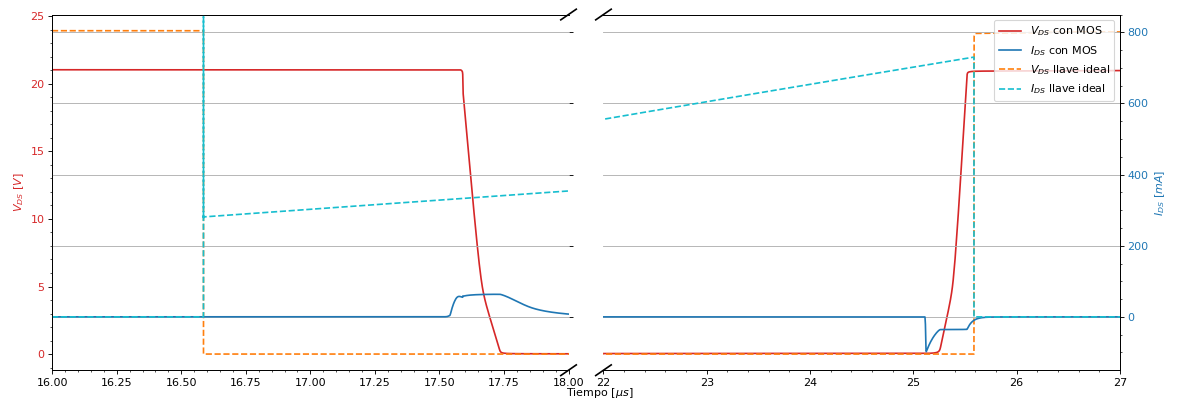
\includegraphics[width=0.9\linewidth]{ImagenesEjercicio-3/ids-vds-2v3}
	\caption{Conmutaciones $V_{ds}$ e  $I_{ds}$.}
	\label{fig:ej3:conmutacionON_OFF_VDS_IDS}
\end{figure}
\begin{figure}[H]
	\centering
	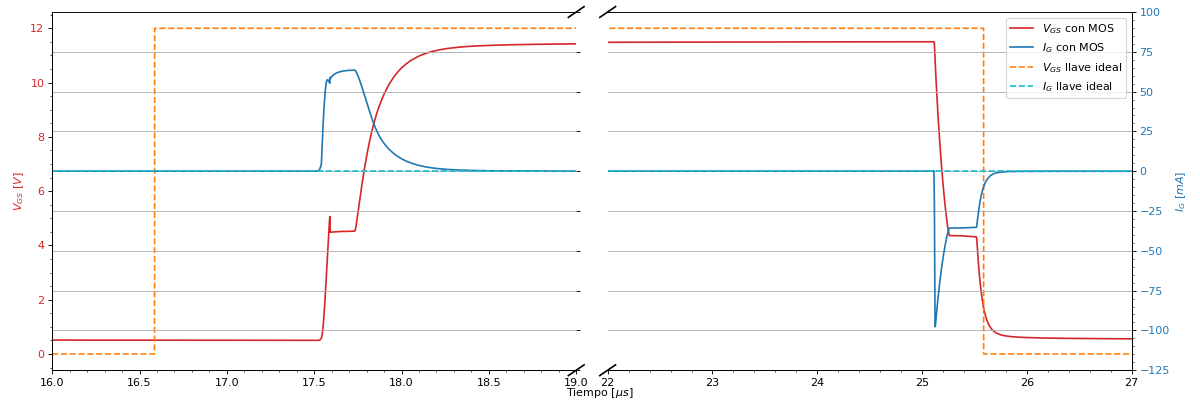
\includegraphics[width=0.9\linewidth]{ImagenesEjercicio-3/ig-vgs-2v3}
	\caption{Conmutaciones $V_{gs}$ e  $I_{g}$.}
	\label{fig:ej3:conmutacionON_OFF_VGS_IG}
\end{figure}
\end{multicols}
\begin{multicols}{2}
\begin{figure}[H]
	\centering
	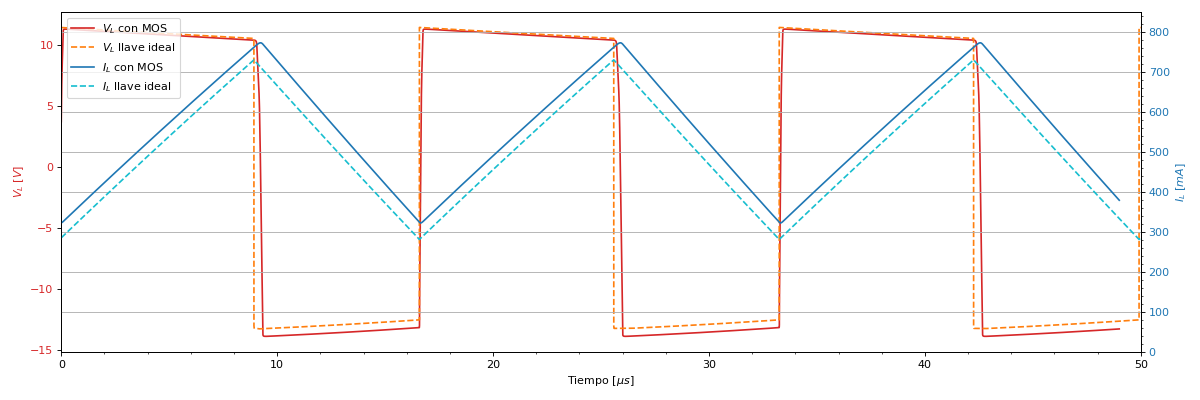
\includegraphics[width=0.9\linewidth]{ImagenesEjercicio-3/il-vl-2v3}
	\caption{Tensión y Corriente sobre la bobina.}
	\label{fig:ej3:Il_Vl}
\end{figure}
\begin{figure}[H]
	\centering
	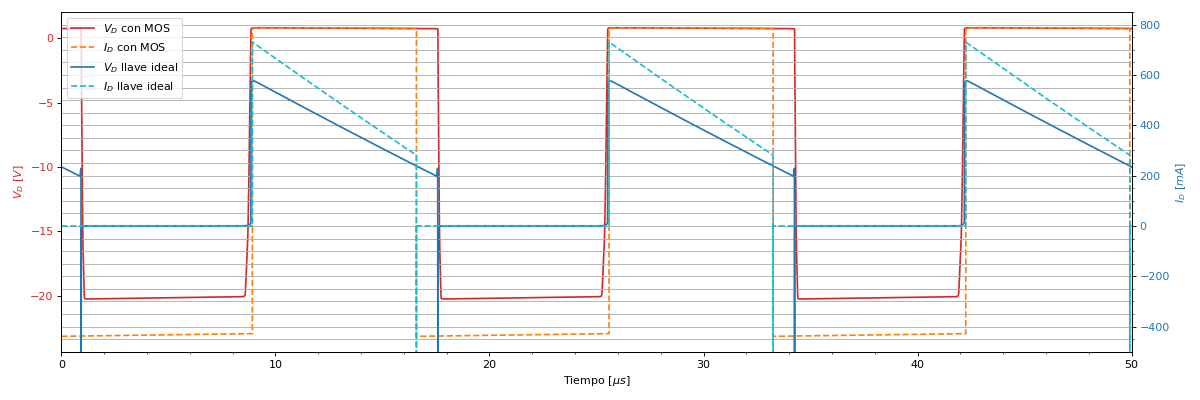
\includegraphics[width=0.9\linewidth]{ImagenesEjercicio-3/id-vd-2v3}
	\caption{Tensión y Corriente sobre el diodo.}
	\label{fig:ej3:Id_Vd}
\end{figure}
\end{multicols}
Al realizar este cambio se puede notar cambios en muchas variables del circuito.
Se  se puede notar un cambio en la $V_L$ y que el duty cycle aumento respecto al que había con un switch idea.
La variacion porcentual del duty cycle es del $\Delta DC  =0.95 \% $
La diferencia en los tiempos de conmutación se debe a que en la llave ideal los cambios son instantáneos mientras que con la real no lo es.
La diferencia entre pendientes en la corriente se debe a la $r_{ds}$ con la que cuenta el mosfet y no la llave. 
También se puede observar que la corriente de reverse recovery del diodo ahora se ve acotada a $I_{rr}\approx 2.8[A]$, la cual es menor a la registrada en el caso anterior.

\subsection{Tiempos de Conmutación}
Los tiempos de conmutación se ven alterados respecto al circuito de la primera sección ya que los valores de $V_{gs-IO}$, $I_{g-IO}$ e $I_{ds}$ dependen principalmente del circuito de aplicación.
en este caso como en la topología Boost cuando el MOS se encuentra abierto se encuentra un circuito RLC mientras que cuando esta cerrado un RL del lado del generador y un RC en la carga esto afectará a los tiempos de $t_{ri}$ $t_{fv}$, $t_{d_{off}}$, $t_{rv}$ y  $t_{fi}$.\\
%\newpage
Algo a notar tanto en el gráfico (\ref{fig:ej3:Id_Vd_SWITCH_BOOST}) y (\ref{fig:ej3:Il_Vl_SWITCH_BOOST}) es que la corriente por la bobina y diodo al igual que la tensión sobre los mismos  depende de la carga, por lo que es razonable que sus valores sean distintos. En cuanto a la corriente de recovery se puede ver que con un MOSFET toma un valor razonable a diferencia que con el componente ideal. 
\begin{multicols}{2}
\begin{figure}[H]
	\centering
	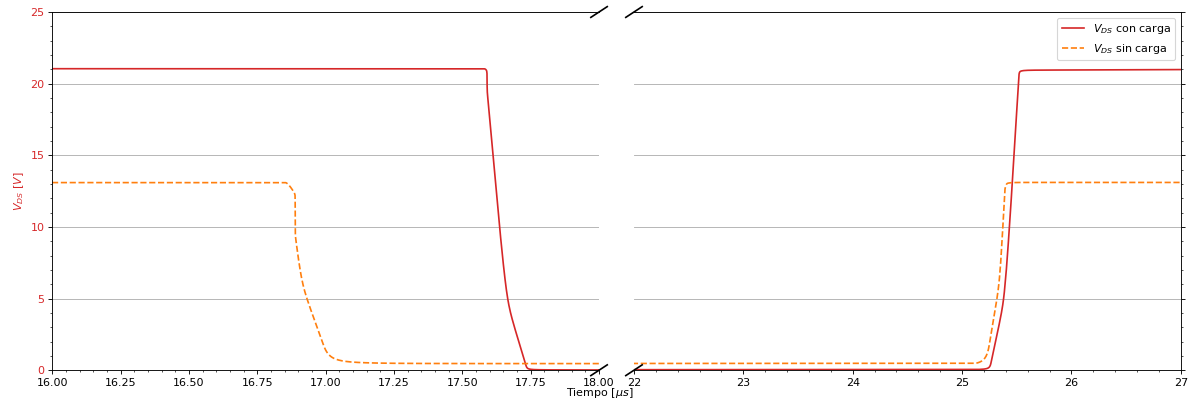
\includegraphics[width=0.9\linewidth]{ImagenesEjercicio-3/ids-vds-1v3}
	\caption{Conmutaciones $V_{ds}$ e  $I_{ds}$ llave con y sin Boost.}
	\label{fig:ej3:conmutacionON_OFF_VDS_IDS_SWITCH_BOOST}
\end{figure}
\begin{figure}[H]
	\centering
	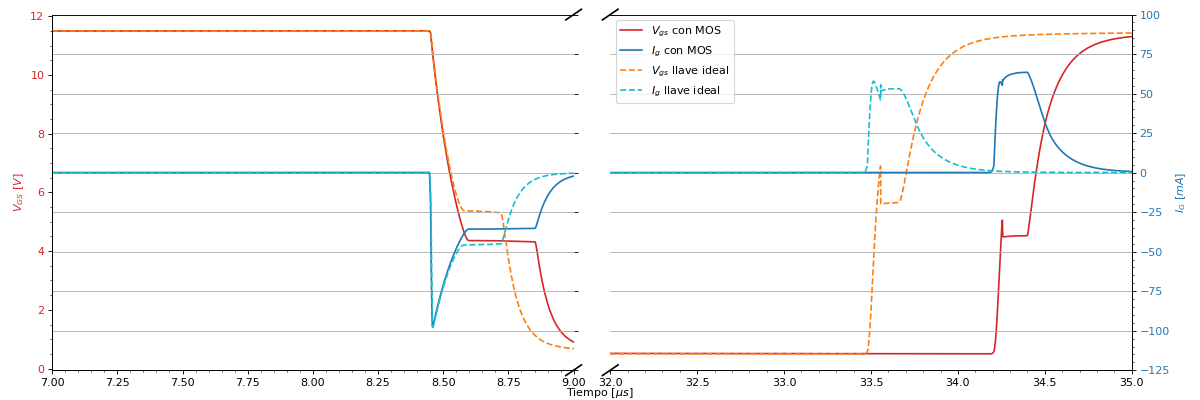
\includegraphics[width=0.9\linewidth]{ImagenesEjercicio-3/ig-vgs-1v3}
	\caption{Conmutaciones $V_{gs}$ e  $I_{g}$ llave con y sin Boost.}
	\label{fig:ej3:conmutacionON_OFF_VGS_IG_SWITCH_BOOST}
\end{figure}
\end{multicols}
\begin{multicols}{2}
\begin{figure}[H]
	\centering
	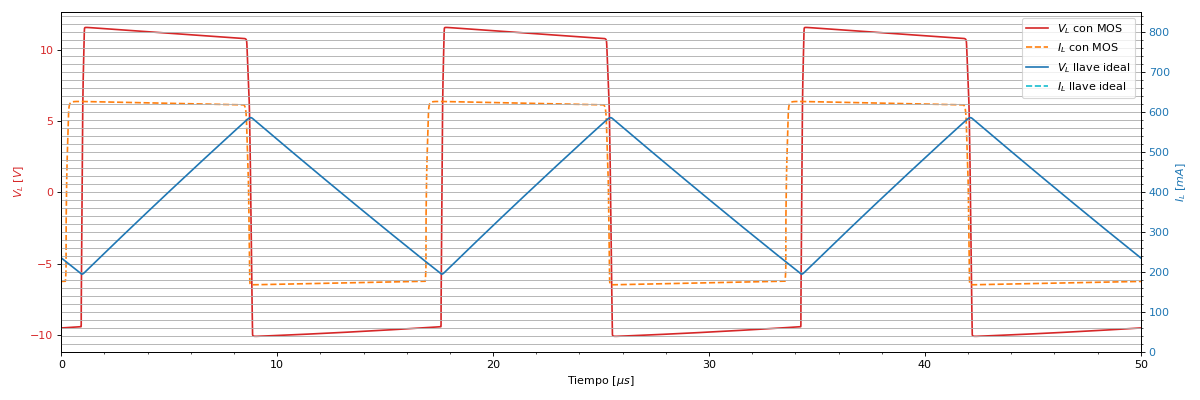
\includegraphics[width=0.9\linewidth]{ImagenesEjercicio-3/il-vl-1v3}
	\caption{Tensión y Corriente sobre la bobina llave con y sin Boost.}
	\label{fig:ej3:Il_Vl_SWITCH_BOOST}
\end{figure}
\begin{figure}[H]
	\centering
	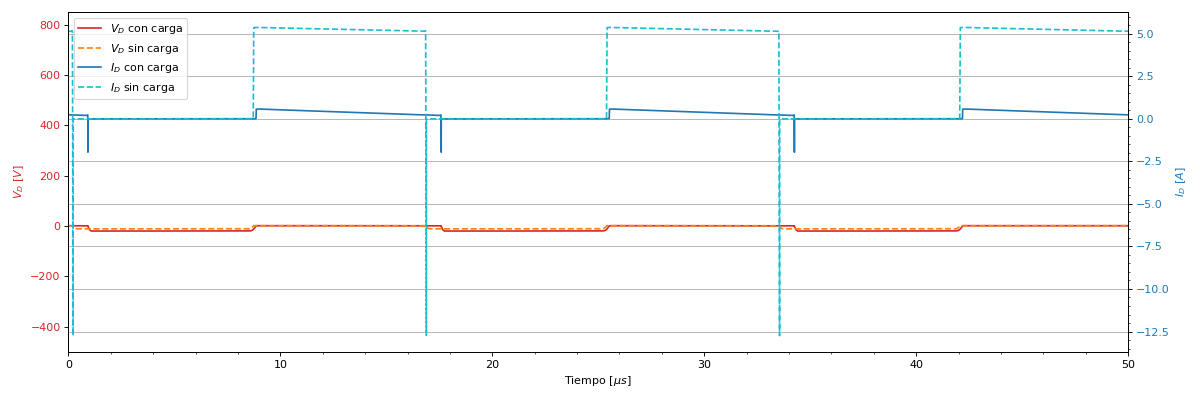
\includegraphics[width=0.9\linewidth]{ImagenesEjercicio-3/id-vd-1v3}
	\caption{Tensión y Corriente sobre el diodo llave con y sin Boost.}
	\label{fig:ej3:Id_Vd_SWITCH_BOOST}
\end{figure}
\end{multicols}

\end{document}